\documentclass[9pt, t]{beamer}
\usepackage[ngerman]{babel} 
\usepackage{textgreek}
\usepackage{amsmath}
\usepackage{amssymb}
\usepackage{mathtools}
\usepackage[
backend=biber,
style=alphabetic,
sorting=ynt
]{biblatex}
\bibliography{presentation.bib}

% Disable navigation buttons
\setbeamertemplate{navigation symbols}{}
\setbeamercovered{transparent}
\newcommand{\margin}{0.05\paperwidth}
\beamersetrightmargin{\margin}
\beamersetleftmargin{\margin}


\title{Approximation von \textpi}
\author{M. van Straten und P. Merz}
\institute{Humboldt-Universität zu Berlin \\
           Sommersemester 2024}
\date{\today}

\usetheme{Berlin}


\begin{document}

\maketitle

\begin{frame}{Inhalt}
    \tableofcontents[pausesections]
\end{frame}

\section{Einführung}

\begin{frame}
    Die Konstante \(\pi\) hat eine natürliche Definition als das Verhältnis
    zwischen dem Umfang und dem Durchmesser eines Kreises.
    \newline\newline
    \textbf{Fundamentaler Bedeutung unter anderem:}
    \begin{itemize}[<+(1)->]
        \item im Gaußschen Integral.
        \item den komplexen Einheitswurzeln.
        \item der Cauchy-Verteilung in der Wahrscheinlichkeitstheorie präsent.
        \item über zahlreiche Disziplinen hinweg.
    \end{itemize}
    \only<6->{
        \(\pi\) ist also eine wichtige Konstanten in der Wissenschaft.
    }
\end{frame}

\begin{frame}{Historie}
    \begin{tabular}{|c||c||c|}
        \hline
        Datum       & Person                          & Korrekte Dezimalstellen \\
        \hline
        ca. 250 v.
        Chr.
                    & Archimedes                      & 2                       \\
        \hline
        1400        & Madhava                         & 10                      \\
        \hline
        1981        & Jean Guilloud                   & 2,000,050               \\
        \hline
        Januar 1988 & \shortstack{Yasumasa Kanada und                           \\ Yoshiaki Tamura} & 201.326.551\\
        \hline
        31.12.2009  & Fabrice Bellard                 & 2,699,999,990,000       \\
        \hline
        14.03.2024  & \shortstack{Jordan Ranous,                                \\
        Kevin O’Brien                                                           \\ und Brian Beeler} & 105,000,000,000,000\\
        \hline
    \end{tabular}
    \cite{Chronology}
\end{frame}

\begin{frame}{Motivation}
    Die Geschichte zeigt: Die genaue Berechnung von \(\pi\) bleibt eine
    mathematische sowie informationstechnische Herausforderung.
    \newline\newline
    \textbf{Ziel dieser Präsentation ist:}
    \begin{itemize}[<+(1)->]
        \item Einführung in mathematische Annäherungsmethoden
        \item \textbf{Analyse in Hinsicht auf:}
              \begin{itemize}[<+(1)->]
                  \item Laufzeit
                  \item Speicherbedarf
                  \item Konvergenzverhalten und Approximationsgenauigkeit
              \end{itemize}
    \end{itemize}
\end{frame}

\section{Theorie}

\subsection{Definitionen}

\begin{frame}{Definitionen}
    \only<1>{%
        \begin{definition}[\(\pi\) in der euklidischen Geometrie]
            Verhältnis zwischen Umfang und Durchmesser eines Kreises
        \end{definition}
        % TODO: cite Analysis I Skript
        Äquivalente Definitionen zum Beispiel in der Analysis über bestimmte
        Nullstellen trigonometrischer Funktionen
    }
    \only<2>{%
        \begin{definition}[Algorithmus]
            % TODO: cite https://de.wikipedia.org/wiki/Algorithmus see citation [1]
            Handlungsvorschrift bestehend aus einer Menge an wohldefinierten
            Schritten
        \end{definition}
        Nützlich, da Algorithmen von Rechnern ausgeführt werden können
    }
    \only<3>{%
        \begin{definition}[Uniforme Teilmenge]
            Eine uniforme Teilmenge \(U\) einer Menge \(M\) ist eine Teilmenge, in der
            jedes Element mit gleicher Wahrscheinlichkeit ausgewählt wird.
            Dies bedeutet, dass für jedes \(x \in M\) die Wahrscheinlichkeit \(P(x \in U)\)
            konstant ist.
        \end{definition}
    }
\end{frame}

\subsection{Annäherungsalgorithmen}

\begin{frame}{Annäherungsalgorithmen}
    \begin{itemize}
        \item Monte-Carlo Simulation
        \item Leibniz-Reihe
        \item Gauß-Legendre Algorithmus
    \end{itemize}
\end{frame}

\begin{frame}{Monte-Carlo Simulation}
    Basierend auf dem Gesetz der Großen Zahl\footnote{Das Gesetz der Großen Zahl
        besagt, dass sich die relative Häufigkeit eines Ereignisses bei großer Anzahl
        von Versuchen dem Erwartungswert annähert.
    } wird versucht, über eine unbekannte Menge \(M\) analytische Aussagen zu treffen,
    indem man sich auf eine endliche uniforme Teilmenge beschränkt.
    \begin{itemize}
        \item<1-> In diesem Fall ist \(M \coloneq \{(x, y) \mid 0 \le x,y \in \mathbb{R} \le 1\}\)
        \item<2-> Mit dem Flächeninhalt eines Kreises folgt, dass
              \begin{equation*}
                  \frac{\pi}{4} = \frac{
                      |\{(x,y) \in M \only<3->{\text{\ mit } \sqrt{x^2 + y^2} \le 1} \}|
                  }{|M|}
              \end{equation*}
              \only<3->{ist.}
        \item<4-> \(\pi\) lässt sich somit approximieren, indem dieses Verhältnis über eine uniforme Teilmenge von \(M\) gebildet wird.
    \end{itemize}
\end{frame}

\begin{frame}{Leibniz-Reihe}
    Durch Ergebnisse der Analysis leitete Leibniz folgedendes Ergebnis her \cite{Leibniz}
    \[ \pi = \sum_{k=0}^{\infty} \frac{(-1)^k}{2k+1} \]
    \uncover<2->{Annäherung von \(\pi\) über \(n\)-te Partialsumme \(\pi \approx \sum_{k=0}^{n} \frac{(-1)^k}{2k+1}\) }
    \begin{itemize}
        \item<3-> Konvergiert sehr langsam, präzise: Sublineare Konvergenz \\
        \item<3-> Benötigt grob 5 Milliarden Terme um auf 10 korrekte Nachkommastellen zu approximieren
    \end{itemize}
\end{frame}

\begin{frame}{Gauß-Legendre}                                                                                                        %https://web.archive.org/web/20080726033059/http://wwwmaths.anu.edu.au/~brent/pd/rpb028.pdf
    \begin{itemize}
        \item<1-> Approximiert \(\pi\) mittels Folgen, die sich des arithmetischen- und geometrischen Mittels zweier Zahlen bedienen
        \item<2-> \( a_0 = 1 \;\;\; b_0 = \frac{1}{\sqrt{2}} \;\;\; t_0 = \frac{1}{4} \;\;\; p_0 = 1 \)
        \item<3-> \( a_{n+1} = \frac{a_n + b_n}{2} \)
        \item<4-> \( b_{n+1} = \sqrt{a_nb_n} \)
        \item<5-> \( t_{n+1} = t_n - p_n(a_n - a_{n+1})^2 \)
        \item<6-> \( p_{n+1} = 2p_n \)
        \item<7-> \(\pi\) wird dann approximiert durch \[ \pi \approx \frac{(a_{n+1} + b_{n+1})^2}{4t_{n+1}} \]
        \item<8-> Konvergiert quadratisch gegen \(\pi\) \cite{Gauß-Legendre}
    \end{itemize}
\end{frame}

\section{Experimente}

\subsection{Laufzeitanalyse}

\begin{frame}
    \textbf{Überblick:}
    \begin{itemize}
        \item Führt Laufzeitanalyse für verschiedene Algorithmen zur
              Approximation von \(\pi\) durch:
              \begin{itemize}
                  \item Leibniz-Reihe, Monte Carlo, Gauss-Legendre, Chudnovsky
              \end{itemize}
        \item Misst Zeit zur Approximation von \(\pi\) auf bestimmte
              Dezimalstellen.
    \end{itemize}

    \visible<2->{
        \begin{figure}<2->
            \centering
            \includegraphics[width=0.6\textwidth]{runtime.png}
            \caption{Laufzeitanalyse und durchschnittliche Zeit pro Stelle für verschiedene Algorithmen zur Approximation von \(\pi\).}
        \end{figure}
    }
\end{frame}

\begin{frame}{Auswertung}
    \begin{itemize}
        \item<1-> \textbf{Leibniz-Reihe}
              \begin{itemize}
                  \item Konvergiert langsam
                  \item Einfache Implementierung
              \end{itemize}
        \item<2-> \textbf{Monte-Carlo Simulation}
              \begin{itemize}
                  \item Zufällige Punktestreuung zur Flächenberechnung
                  \item Konvergenz verbessert sich mit Anzahl der Punkte
              \end{itemize}
        \item<3-> \textbf{Gauss-Legendre Algorithmus}
              \begin{itemize}
                  \item Schnelle Konvergenz
                  \item Komplexere Implementierung
              \end{itemize}
        \item<4-> \textbf{Chudnovsky Algorithmus}
              \begin{itemize}
                  \item Extrem schnelle Konvergenz
                  \item Sehr komplexe Implementierung
              \end{itemize}
    \end{itemize}
\end{frame}

\subsection{Konvergenz}

\begin{frame}{Daten}
    \begin{figure}
        \begin{center}
            \leavevmode
            \onslide<1>\includegraphics[width=\textwidth]{runtime.png}
            \onslide<2>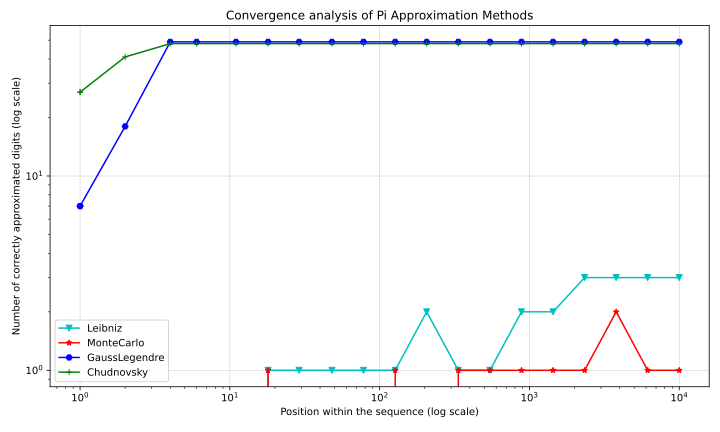
\includegraphics[width=\textwidth]{convergence.png}
        \end{center}
    \end{figure}
\end{frame}

\begin{frame}{Auswertung und Zusammenfassung}

\end{frame}

\subsection{Präzision}

\subsection{Speicherbedarf}

\begin{frame}{Literaturverzeichnis}
    \printbibliography
\end{frame}

\end{document}
